
\documentclass{article}
\usepackage{spconf,amsmath,amssymb,cite}
\usepackage{graphicx}
\usepackage{color}
\usepackage{hyperref}
\usepackage{cleveref}

% Title.
% ------
\title{Exploiting Harmonics with Convolutional Neural Networks}

% Note: Please do NOT use \thanks or a \footnote in any of the author markup

% Single address
% To use with only one author or several with the same address
% ---------------
%\oneauthor
% {Names should be omitted for double-blind reviewing}
% {Affiliations should be omitted for double-blind reviewing}

% Two addresses
% --------------
%\twoauthors
%  {First author} {School \\ Department}
%  {Second author} {Company \\ Address}

%% To make customize author list in Creative Common license, uncomment and customize the next line
%  \def\authorname{First Author, Second Author}


% Three addresses
% --------------
\twoauthors%
  {First Author} {Affiliation1 \\ {\tt author1@ismir.edu}}
  {Second Author} {\bf Retain these fake authors in\\\bf submission to preserve the formatting}
%  {Third Author} {Affiliation3 \\ {\tt author3@ismir.edu}}

%% To make customize author list in Creative Common license, uncomment and customize the next line
%  \def\authorname{First Author, Second Author, Third Author}

% Four or more addresses
% OR alternative format for large number of co-authors
% ------------
%\multauthor
%{First author$^1$ \hspace{1cm} Second author$^1$ \hspace{1cm} Third author$^2$} { \bfseries{Fourth author$^3$ \hspace{1cm} Fifth author$^2$ \hspace{1cm} Sixth author$^1$}\\
%  $^1$ Department of Computer Science, University , Country\\
%$^2$ International Laboratories, City, Country\\
%$^3$  Company, Address\\
%{\tt\small CorrespondenceAuthor@ismir.edu, PossibleOtherAuthor@ismir.edu}
%}
%\def\authorname{First author, Second author, Third author, Fourth author, Fifth author, Sixth author}


%\sloppy % please retain sloppy command for improved formatting

\def\eg{\emph{e.g.}}
\def\ie{\emph{i.e.}}
\def\etc{\emph{etc.}}
\def\etal{\emph{et al.}}


\begin{document}

%
\maketitle
%
\begin{abstract}

% Convnets have rocked MIR
Convolutional neural networks have shown great performance across a variety of tasks in audio analysis.
% Operate on time-freq reps, which are not images
In vision applications, convolutional networks exploit statistical regularities in spatial locality, \ie, neighboring pixels.
%By limiting the receptive field of a filter to a spatial neighborhood, a convolutional network can learn representations which are position-invariant by allowing filters to move along spatial dimensions.
However, in audio, these models often operate on time-frequency representations, which exhibit different statistical regularities from natural images.
% Sound is harmonic, and model assumptions may not hold.
Although time-frequency representations exhibit local regularities, modeling only these interactions ignores the relationships between harmonically related frequencies, which appear distant in time-frequency representations.
% Make input rep harmonic, does it matter?
To better adapt convolutional networks to audio, we craft an alternative input representations that directly exploits harmonic frequency statistics.
%and determine what effect these have on the efficacy of the learned model.
% How do we do it?
We study this approach in a large, solo instrument classification task, and examine how model architecture influences performance.
% What do we find?
%Experimental results show that the use of harmonic convolutions leads to better generalization, faster computation time, and more compact models per unit of performance.
% Closeout
Finally, we provide an open source framework to reproduce our dataset and experimental results.
\end{abstract}

\begin{keywords}
    audio, deep learning, instrument recognition, music
\end{keywords}
\section{Introduction}\label{sec:introduction}

% Deep learning, so hot right now... deep learning.
%Many tasks in audio analysis aim to develop computational systems for modeling the human perception of acoustic signals to achieve robust content understanding at scale, \eg, tens of millions of tracks.

Over the last decade, many research communities have embraced automatic feature learning and deep networks as a viable and superior alternative to hand-crafted feature design.
In particular, convolutional neural networks (CNNs)~\cite{lecun1998gradient} excel at modeling complex, nonlinear, and multi-scale behavior found in acoustic signals.
CNNs are now an common choice for many audio analysis tasks, such as speech recognition, environmental event detection and scene classification, and a host of musical analysis tasks, such as chord estimation, rhythm analysis, structural segmentation, or instrument detection.
%TODO: cite application papers

\subsection{CNNs and spatial locality}
It is worth noting that convolutional networks draw inspiration from biological vision systems~\cite{hubel1964effects}, and common model architectures have been designed with computer vision in mind.
In vision applications, CNNs exploit two fundamental properties of natural images:
one, statistical regularities exist primarily within small spatial regions (distant pixels tend to be uncorrelated),
and two, weights over local receptive fields can be shared across spatial dimensions, providing translation-invariant features.

While these properties have been empirically demonstrated to hold for natural images, it is not immediately obvious that the same would be true for time-frequency representations of audio.

%We can visualize why this is a good idea.
Here, we take the CIFAR10 dataset~\cite{krizhevsky2009learning}, which consists of ${32\times 32}$ images.
We use the training set of 25K images, compute a two-dimensional auto-correlation between each image and a slightly cropped version of itself, and average over the dataset.
As expected, \Cref{fig:image_corr} illustrates that neighboring pixels are better correlated than those at a distance, and there is little observable bias in either dimension.

In audio, time-frequency representations (\eg, magnitude spectrograms) are not images, but much of the existing literature applies the same image-based CNN methods.
This raises an interesting question: how do the statistical regularities of spectrograms differ from those of natural images?

We therefore repeat the autocorrelation experiment, but instead draw observations from constant-Q transform (CQT) representations of audio.
Using the librosa toolkit~\cite{librosa041}, we computed CQT spectra over a number of recordings in the USPop dataset~\cite{berenzweig2004large} and drew 25K windowed observations uniformly at random.
As before, the valid, two-dimensional auto-correlation is performed between each windowed observation and a cropped version of itself.
\Cref{fig:cqt_corr} demonstrates there are two notable differences from \Cref{fig:image_corr}.
First, consistent with our intuition, the CQT representation exhibits strong correlations with harmonically related frequencies, being the octave (2:1), fifth (3:2), and major third (4:3).
Second, these correlations are not symmetric in frequency.

\begin{figure}
\label{fig:cqt_corr}
\end{figure}

\begin{figure}
\label{fig:image_corr}
\end{figure}

\subsection{Our contributions}
In this work, we develop Harmonic Convolution Neural Networks (HCNNs), and apply the method to the task of solo music instrument classification.
To evaluate the method, we developed a newly standardized dataset referred to the Music INSTrument (MINST) dataset.
%The remainder of the paper is organized as follows:
%Section II details our approach to exploiting correlations in convolutional networks;
%Section III describes the experimental method used in this work;
%and Section IV discusses results and conclusions drawn therein.


\section{Sparsity in Convolutional Networks}\label{sec:page_size}

% 1. convnets in time-frequency (stft, 1d)
% 2. convnets in time-logf (cqt, 1d/full)
% 3. convnets in time-logf (cqt, 2d/small)
% 4. lostanlen: octave relations
% 5. us: harmonic relations

\begin{figure}
    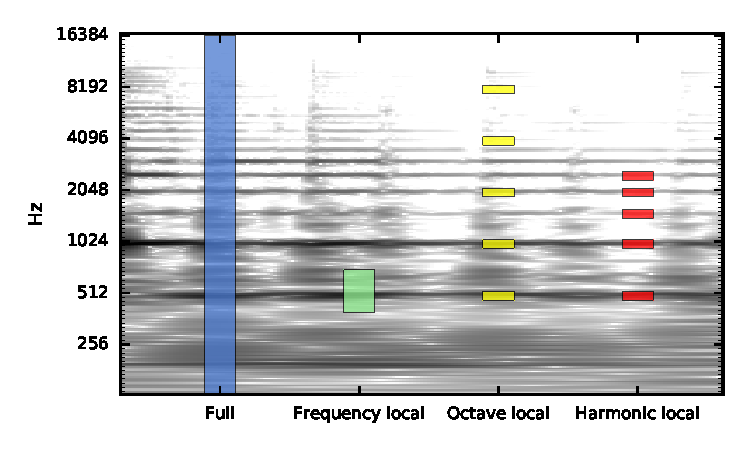
\includegraphics[width=\columnwidth]{figs/filter-shapes}
    \caption{A comparison of different sparsity patterns for convolutional networks on spectrogram inputs.
        \emph{Full} connectivity (blue) requires that the filter connect to all frequency bins in a temporal window around the center frame.
        \emph{Frequency-local} connectivity (green) only connects a filter to near-by frequencies.
        \emph{Octave-local} connectivity (yellow) allows a filter to connect to the same pitch classes across different octaves.
        \emph{Harmonic-local} connectivity (red) allows a filter to connect to harmoincally related frequencies.}
\label{figs:filter-shapes}
\end{figure}
Convolutional neural networks (CNNs) derive their expressive power by modeling ``local'' statistical regularities.
As illustrated in \Cref{figs:filter-shapes}, there are a variety of ways to model ``locality'' in spectrogram representations.

Arguably the simplest method is to model the entire frequency range over a short time window.  
This method, denoted as \emph{Full} in \Cref{figs:filter-shapes} requires filter coefficients which span the entire frequency axis of the spectrogram.
While this model makes the fewest possible assumptions about independence among frequencies, it also cannot be made pitch-invariant since the filter cannot move along the frequency axis.
Consequently, it may take a large number of filters --- each with a large number of coefficients --- and thus a large amount of training data to model the relatively simply phenomenon of pitch modulation.
However, this approach has been demonstrated to be effective for high-level tasks. %TODO: cite sander, maybe pablo, eric, etc\ldots

The second approach uses smaller filters, which can be moved along the frequency axis.
For this approach to properly generate pitch-invariant features, the frequency axis of the spectrogram must be logarithmically spaced, as in the constant-Q transform (CQT).
This method, denoted as \emph{Frequency-local} in \Cref{figs:filter-shapes}, is closely related to the local receptive field filters used in computer vision applications.
Frequency-local filters can therefore capture highly localized characteristics of sound, such as attack profile or vibrato, but cannot directly capture properties derived from distant frequencies, such as timbre.
Higher-level properties can be modeled by subsequent processing layers, and this approach has been shown to be effective for intermediate-level tasks such as instrument recognition. %self-cite. TODO: eric, did you use this for chords?


Recently, Lostanlen and Cella~\cite{lostanlen2016} proposed a variant of the Frequency-local approach in which filters are connected to small time-frequency patches tiled across multiple octaves.
This method is depicted in \Cref{figs:filter-shapes} as \emph{octave-local}.
As the illustration shows, this connectivity scheme allows for a filter to be pitch-invariant while modeling local time-frequency statistics as well as broad spectrum properties.
Consequently, this approach --- when used in combination with the previous two methods --- demonstrated superior performance for instrument recognition, which requires both pitch-invariance and broad-spectrum models.
Note, however, that connections are only included to frequencies related by an integer power of 2 to the bottom time-frequency patch.
Octave-local design therefore disregards odd harmonics, which can be highly informative for determining the timbre of a sound.
%We also note that Lostanlen's implementation limited the octave neighborhood to span three octaves.

%Reference Lostanlen's ISMIR work.
%The facets we consider differently are...

\subsection{Harmonic CNNs}

The proposed harmonic CNN (HCNN) is a straightforward extension of the previous methods.
Rather than connect a filter to time-frequency patches which are in octave relation to each other (as in the octave-local model), the HCNN connects time-frequency patches which are related by integer multiples.
This connectivity pattern is illustrated in the final column of \Cref{figs:filter-shapes} (harmonic-local).
Note that the harmonic-local pattern is able to capture the odd harmonics (third and fifth)  of the fundamental (around 500Hz) which are missed by the frequency- and octave-local models.

\subsection{HCNN Implementation}

Formally, we define the HCNN operation as a function parametrized by coefficients $w \in \mathbb{R}^{F \times T \times H}$, where $F$ denotes the number of frequency bins, $T$ denotes the number of time frames, and $H$ denotes the number of harmonics to model:
\begin{equation}
    {g_w(X)}_{t, k} := 
    \sum_{\substack{%
        h \in \{1, 2, \ldots, H\}\\
        i \in \{-\lfloor T/2\rfloor, \ldots, \lfloor T/2 \rfloor\}\\
        j \in \{-\lfloor F/2\rfloor, \ldots, \lfloor F/2 \rfloor\}}
    }
    \hspace{-3em}%
    w_{ijh} \cdot X^h\left(t + i,\; k + j\right)\label{eq:hcnn}
\end{equation}
where $X^h(t, k)$ denotes the $h$th harmonic of frequency at bin $k$ and time $t$.

% Octave-local is easy: just wrap the cqt
Note that the octave-local model can be recovered from \cref{eq:hcnn} by taking a subset of harmonics $h=2^n$ for integer $n$.
For a CQT with $B$ bins per octave and minimum basis frequency $f_{\min}$, we have bases frequencies defined by
\begin{equation}
    f_k = 2^{k/B} \cdot f_{\min}, \label{eq:cqtfreqs}
\end{equation}
and for any $f_k$, its $2^n$ harmonic will be located at $f_{k + (n-1)\cdot B}$.
The octave-local model can therefore be implemented efficiently by standard 2-dimensional CNN frameworks by reshaping the CQT into a three-dimensional array parametrized by (time, pitch class, octave number).\footnote{To avoid boundary effects, Lostanlen and Cella use a redundant encoding where the ``pitch class'' dimension spans more than one octave.}
The octave dimension thus plays a role similar to color channels in image processing, since the selected harmonics align exactly along the ``octave'' dimension.

% Harmonic is trickier, since the spacing is not fixed in CQT space
The general harmonic CNN is somewhat more difficult to implement.
The $h$th harmonic of a frequency $f_k$ will not generally coincide with an integer bin index $j$, since this would require
\begin{eqnarray}
    f_j = 2^{j/B} \cdot f_{\min} &=& h \cdot 2^{k/B}\cdot f_{\min} = h \cdot f_k \notag \\
    % 2^{j/B} = h * 2^{k/B}
    % j/B = log_2 h + k/B
    % j = k + B log_2 h
\Rightarrow \quad j &=& k + B \cdot \log_2 h,
\end{eqnarray}
which is not an integer for $h \neq 2^n$.
\Cref{eq:hcnn} cannot be directly implemented on a CQT without resorting to some form of approximation (\eg, interpolation between frequency bands).
Moreover, because the harmonically related bins are not uniformly spaced along the frequency axis, there is no simple reshaping of the spectrogram that would simultaneously align patches for use with standard 2D convolution operators.

% Solution: use harmonic planes! analogous to color channels
%           + volumetric filters
Instead of octave-wrapping, we generate $H$ constant-Q transforms $X^1, X^2, \dots, X^H$ for a given input signal.
$X^1$ is defined as a CQT with minimum basis frequency $f^1_{\min}$.
For $h > 1$, we scale the minimum basis frequency to
\begin{equation}
    f^h_{\min} := h \cdot f^1_{\min}.\label{eq:fmin}
\end{equation}
By the definition of the CQT, the subsequent basis frequencies also scale by a factor of $h$ in relation to the original:
\begin{eqnarray}
    f^h_k &=& 2^{k/B} \cdot f^h_{\min}\\
        &=& 2^{k/B} \cdot h \cdot f^1_{\min}\\
    &=& h \cdot f^1_k.
\end{eqnarray}
This implies that for all frequency bins $k$, the $h$th harmonic of $X^1_{t, k}$ is located at $X^h_{t, k}$, as illustrated in \Cref{fig:hcnn}.
Collecting all ${(X^h)}_{h=1}^H$ into a three-dimensional array indexed by (time, frequency, harmonic) thus preserves index locality, and \cref{eq:hcnn} can be computed with standard 2-dimensional CNN frameworks.


\begin{figure}
    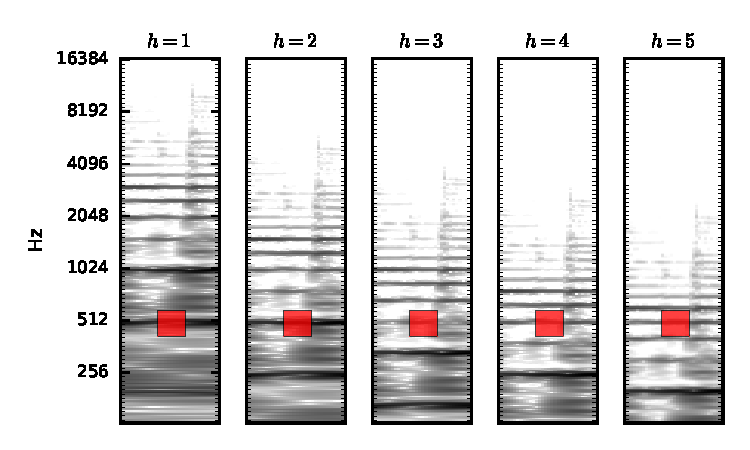
\includegraphics[width=\columnwidth]{figs/hcnn}
    \caption{The HCNN is implemented by generating $H$ constant-Q transforms $X^1, X^2, \ldots, X^H$.
    A single HCNN filter connects to the same time-frequency indices across all harmonic channels (indicated in red), just as color image filters connect to the same spatial coordinates across all color channels.}
\label{fig:hcnn}
\end{figure}

\section{Method}\label{sec:typeset_text}

%The width (time) of the filters should match that of MH: above I suggested 5x5, but I think 7x7 might be better since it captures +- 1 semitone from the center bin. In M2, this translates to +- 3 semitones. For MF, layer 1 will be full-height by 7.

%For layer 2 in MF, the input will have shape (n[1], 1, T - 7//2); frequency information is collapsed out by valid-mode convolution, and we effectively have two-dimensional data (filter number, time). Layer 2 filters then must have shape like (1, width), and the width may as well match the width of layer 2 in MH/M2 (I suggested 9x9 above).

%After that, we max-pool over time and feed into dense layer just as in the other architectures.



\subsection{The MINST Dataset}\label{subsec:body}

% Issues with audio datasets
Training and evaluating supervised machine learning approaches on MIR tasks faces a near-universal issue of data.
% Not many open-audio datasets that can be shared.
While many researchers have built or leveraged labeled collections of audio, concerns of copyright undermine the reproducibility of results.
% Data integrity issues, many MIR tasks are subjective, raising issues of evaluation and the use of ground truth.
In many instances though, collections that do provide access to audio data suffer from questions of validity and integrity, such as GTZAN~\cite{tzanetakis2002musical,sturm2012analysis}, or focus on subjective tasks which raise issues of ``ground truth''.
% Seldom large in size
Complementing these issues, large, well-annotated audio datasets are uncommon.
These challenges make it difficult to form robust conclusions across experiments and researchers.

Sizeable, open, and objective of datasets like MNIST~\cite{lecun1998mnist} or CIFAR~\cite{krizhevsky2009learning}, however, have served the computer vision community well in the last two decades, helping lead to a number of breakthroughs in the field.
It is hard to imagine, for example, where the community would be without the early role served by MNIST.\@
Here, we strive to develop a similarly standardized data by building on top of previous efforts in the MIR community to build collections of solo instrument samples.

Here, we combine a number of open datasets in a common manner to yield the Music Instrument dataset, dubbed MINST\footnote{\url{http://github.com/ejhumphrey/minst-dataset}}, in honor of its handwritten digit counterpart.
Note onsets are annotated semi-automatically;
a number of onset detection methods are applied, and subsequently verified or corrected manually, as needed.
These reference note onsets are then used to segment longer recordings into individual notes.
Here, each note is trimmed to a constant 1-second duration; where observed notes are shorter than this, a -65dBFS Gaussian noise signal is appended.
This results in nearly 39k note observations from 13 instrument classes, spanning 3 different corpora:
UIowa Music Instrument Samples\footnote{}, RWC\footnote{}, and Philharmonia\footnote{}.
The data used herein is made freely available online\footnote{}.


\subsection{Evaluation}



\subsection{Experimental Design}

Please include the copyright notice exactly as it appears here in the lower left-hand corner of the page.
It is set in 8pt Times.


\section{Discussion}

First level headings are in Times 10pt bold,
centered with 1 line of space above the section head, and 1/2 space below it.
For a section header immediately followed by a subsection header, the space should be merged.

\subsection{Second Level Headings}

Second level headings are in Times 10pt bold, flush left,
with 1 line of space above the section head, and 1/2 space below it.
The first letter of each significant word is capitalized.

\subsubsection{Third and Further Level Headings}

Third level headings are in Times 10pt italic, flush left,
with 1/2 line of space above the section head, and 1/2 space below it.
The first letter of each significant word is capitalized.

Using more than three levels of headings is highly discouraged.


% For bibtex users:
\bibliographystyle{IEEEbib}
\bibliography{references}
\end{document}

